\documentclass[12pt,hyperref={pdfpagelabels=false},notes=show]{beamer}

\usetheme[]{FFF}

% Bugfix for pdfpagelables=false
\providecommand\thispdfpagelabel[1]{}

% Standard packages

\usepackage[english,ngerman]{babel}
\usepackage[utf8]{inputenc}
\usepackage{times}

% Setup TikZ

\usepackage{tikz}
\usetikzlibrary{arrows}
\tikzstyle{block}=[draw opacity=0.7,line width=1.4cm]

% Text \us
\usepackage{textcomp}
\usepackage{mathcomp}

% Textpos
\usepackage[absolute,overlay]{textpos}
\setlength{\TPHorizModule}{\paperwidth}
\setlength{\TPVertModule}{\paperheight}

% Blitz-Symbol
\usepackage{stmaryrd}

% Tabellen
\usepackage{multirow}
\usepackage{array}
\usepackage{colortbl}
\definecolor{lightblue}{rgb}{ 0.55, 0.55, 1.00}
\definecolor{lightred}{rgb}{  1.00, 0.35, 0.35}
\definecolor{lightgreen}{rgb}{0.50, 1.00, 0.50}
\newcommand{\ccg}{\cellcolor{lightgreen}}
\newcommand{\ccr}{\cellcolor{lightred}}
\newcommand{\ccb}{\cellcolor{lightblue}}

% Listings
\usepackage{listings}

\setlength{\parindent}{0cm}

% Stroke
\usepackage{ulem}

% vc
\input{vc.tex}

%%%%%%%%%%%%%%%%%%%%%% /LAYOUT %%%%%%%%%%%%%%%%%%%%%%%%%%%%


% Author, Title, etc.

\title{Aktuelles vom Wireless Mesh Netz}

\subtitle{Erlanger Linuxtag 2016}

\author[Tim Niemeyer]{Tim Niemeyer {\tiny \textless{}tim@freifunk-franken.de\textgreater{}}\texorpdfstring{\tiny \\\\
                        https://github.com/RedDog99/vortrag-erlug2016.git\newline
                        \VCRevisionMod}{}}

\date[30.04.2016]{30.4.2016}

\newcommand{\zb}{z.\,B.\@}
\newcommand{\us}{~\textmu{}s}
\newcommand{\uv}{~\textmu{}V}
\newcommand{\ms}{~ms}

\begin{document}

\usebackgroundtemplate{
\includegraphics[height=\paperheight,width=\paperwidth]{slides_background_title}}

\beamertemplatenavigationsymbolsempty
\begin{frame}[plain,squeeze]
	\maketitle
\end{frame}\addtocounter{framenumber}{-1}

\usebackgroundtemplate{
\includegraphics[height=\paperheight,width=\paperwidth]{slides_background}}

\begin{frame}{Inhalt}
    \hspace{0.1\textwidth}
    \parbox[c][0.8\textheight][s]{0.8\textwidth}{
        \tableofcontents
    }
\end{frame}

%%%%%%%%%%%%%%%%%%%%%% CONTENT %%%%%%%%%%%%%%%%%%%%%%%%%%%%

\section{Freifunk}

\begin{frame}{Einleitung}
    \begin{itemize}
        \item Freifunk Franken ist lokaler Ableger der Freifunk-Bewegung (freifunk.net)
        \item Nicht-kommerzielle Initiative für freie Funknetzwerke\\
        \begin{itemize}
            \item[$\rightarrow$] Bürger investieren in Eigenregie Zeit, Geld und Enthusiasmus
        \end{itemize}
        \item Nicht nur \glqq{}kostenloses Internet\grqq $\Rightarrow$ \glqq{}freies Netzwerken\grqq\\
        \begin{itemize}
            \item Lokal intressante Dienste zur Verfügung stellen (Webcams)
            \item Text, Musik und Filme über das interne Freifunk-Netz übertragen
            \item Über lokale Dienste Chatten oder Telefonieren
        \end{itemize}
    \end{itemize}
\end{frame}

\begin{frame}{Wie es funktioniert}
    \begin{itemize}
        \item Freifunker stellen WLAN-Router für sich selbst und den Datentransfer der anderen Teilnehmer zur Verfügung
        \begin{itemize}
            \item ggf. mit Anschluss an das www (für VPN)
        \end{itemize}
        \item Benachbarte Router verbinden sich und spannen ein sogenanntes Mesh-Netzwerk auf
        \item Nicht benachbarte Router verbinden sich mittels VPN-Tunnel zum Freifunk
        \item Jegliche Verbindung ins www wird hierüber umgeleitet, um Risiken der Störerhaftung zu entgehen
    \end{itemize}
\end{frame}

\begin{frame}{Was braucht man?}
    \begin{itemize}
        \item Ein günstiger, unterstützter Router (ab ca. 17€)
        \item Eine spezielle Firmware
        \item Die Zustimmung zum \glqq{}Pico-Peering Agreement\grqq
        \begin{itemize}
            \item Regelwerk, das grundsätzliche Eigenschaften eines Freifunk-Netzwerkes sichert
            \begin{enumerate}
                \item Freier Transit
                \item Offene Kommunikation
                \item Keine Garantie (Haftungsausschluss)
                \item Nutzungsbestimmungen
                \item Lokale (individuelle) Zusätze
            \end{enumerate}
            \item Die Freifunk Firmware implementiert diese Grundsätze standardmäßig
        \end{itemize}
    \end{itemize}
\end{frame}


\section{Grundlagen}
\begin{frame}{}
    \begin{center}
        Grundlagen
     \end{center}
\end{frame}

\begin{frame}{Ein typisches Freifunk Netz}
    \begin{itemize}
        \item Ein Batman-Adv Netz
        \begin{itemize}
            \item[$\rightarrow$] "Wie ein großer dezentraler Switch"
        \end{itemize}
        \item VPN für die Funkinseln
        \begin{itemize}
            \item Multi-Client zu Multi-Client VPN
            \item Layer-II Netz
            \item Kein internes Routing / Forwarding
        \end{itemize}
        \item Mehrere VPN Server / Gateway
        \begin{itemize}
            \item DHCP
            \item DNS Namensauflösung
            \item Gateway zum Internet / ICVPN
        \end{itemize}
        \item Monitoring
        \begin{itemize}
            \item Karte aller Knoten
        \end{itemize}
    \end{itemize}
\end{frame}

\begin{frame}{Ein typisches Freifunk Netz}
    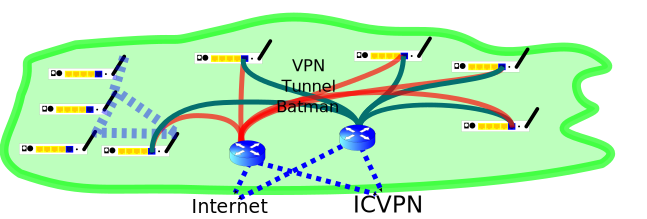
\includegraphics[width=\textwidth]{img/svg/freifunk_konzepte_alt.pdf}
\end{frame}

\begin{frame}{Freifunk Franken Netz}
    \includegraphics[width=\textwidth]{img/svg/freifunk_konzepte.pdf}

    \begin{itemize}
        \item Mehrere Layer-2 Inseln (Hoods)
        \item Verbindung per Layer-3
        \item Dezentrale Gateways
    \end{itemize}
\end{frame}

\begin{frame}{Knoten VPN}
    \begin{itemize}
        \item Verwendetes VPN: fastd
        \begin{itemize}
            \item n:m VPN
        \end{itemize}
        \item Endpunkt Vermittlung über KeyXchange:
        \begin{itemize}
            \item Zentrale Webseite \only<2-3>{{\color{red}Problem!}}
            \item Knoten meldet sich mit Standort
            \item Geographisch nächste Hood wird zugewiesen (voronoi)
            \item Client bekommt Liste aller Server der Hood
        \end{itemize}
        \item<3> Keine weitere Unterscheidung zu welcher Hood der Knoten gehört
        \item<3> {\color{red}Problem!} Funk Verbindung zwischen den Hoods
    \end{itemize}
\end{frame}

\begin{frame}{VPN Server}
    \begin{itemize}
        \item VPN Server: In jeder Hood gibt es mehrere davon
        \item Hoodzuweisung manuell im KeyXchange
        \item DHCP
        \begin{itemize}
            \item Aktuell ausschließlich IPv4
            \item Unterschiedliche Latenzen: Ungleiche Server Auslastung
            \begin{itemize}
                \item[$\rightarrow$] Batman-Adv GW Selection
                \item Anpassung nach Traffic Auslastung
            \end{itemize}
        \end{itemize}
        \item DNS Namesauflösung
        \item Policy base routing
        \item VPN (GRE) Tunnel zu anderen Gateways
        \begin{itemize}
            \item OLSR Routing
        \end{itemize}
    \end{itemize}
\end{frame}

\begin{frame}{Gateways}
    \begin{itemize}
        \item Verbindet Freifunk und Internet
        \item IPv4 NAT (oft übers Ausland) ins Internet
        \item Announced 0.0.0.0/0 via OLSR
        \begin{itemize}
            \item Dynamic Gateway Plugin
            \item VPN Server können diese Routen nutzen
        \end{itemize}
        \item Routing Metrik ohne Traffic/Bandbreite
        \item<2> {\color{red}Problem!} Ungleiche Traffic Verteilung
    \end{itemize}
\end{frame}

\section{Historie}
\begin{frame}{}
    \begin{center}
        Als Ausschnitt:\\
        Das Netz Anfang des Jahres
     \end{center}
\end{frame}

\begin{frame}{Freifunk Knoten}
    \begin{itemize}
        \item Ziel: Ohne Konfiguration
        \begin{itemize}
            \item Keine DHCP Ranges
            \item LAN Ports vorkonfiguriert
            \item Ausnahme: Passwort für root Login
        \end{itemize}
        \item Hat nur eine Link-Local IPv6 Adresse
        \item Batman-Adv 2013 (!)
    \end{itemize}
\end{frame}

\begin{frame}{Netmon}
    \begin{itemize}
        \item Nodewatcher
        \begin{itemize}
            \item Generiert Status-Daten
            \item XML
            \item alle 5 Minuten
        \end{itemize}
        \item Configurator
        \begin{itemize}
            \item Verknüpft Netmon und Knoten
        \end{itemize}
        \item Crawler
        \begin{itemize}
            \item Sammelt Status-Daten
            \item Download über http Schnittstelle der Knoten
            \item Alles über Link-Local
            \begin{itemize}
                \item Muss in jeder Hood drin sein
            \end{itemize}
        \end{itemize}
        \item Netmon
        \begin{itemize}
            \item Visualisiert Status-Daten
            \item Mit den vielen Crawls hoffnungslos überfordert
        \end{itemize}
    \end{itemize}
\end{frame}

\begin{frame}{Monitoring}
    \begin{itemize}
        \item Alfred
        \begin{itemize}
            \item XML
            \item alle 5 Minuten
            \item Multicast
        \end{itemize}
        \item Multicast Daten können auf mehreren Gateways gelesen werden
        \item Die Daten können von dort an eine zentrale Webseite (Karte, etc.) geschickt werden
        \item Standort und Ansprechpartner wird aus dem Netmon geladen
        \item Problem: Abhängig vom Netmon
    \end{itemize}
\end{frame}

\begin{frame}{Freifunk Knoten}
    \begin{itemize}
        \item Ziel: Ohne Konfiguration
        \begin{itemize}
            \item Keine DHCP Ranges
            \item LAN Ports vorkonfiguriert
            \item Ausnahme: Passwort für root Login
        \end{itemize}
        \item Hat nur eine Link-Local IPv6 Adresse
        \item Nur SSH Zugang
        \begin{itemize}
            \item[$\rightarrow$] Kein Webinterface
        \end{itemize}
        \item Batman-Adv 2013 (!)
    \end{itemize}
\end{frame}

\begin{frame}{Firmware Bau}
    \begin{itemize}
        \item Basiert auf OpenWrt
        \item ,,Eigenes'' Framework (Buildscript)
        \item Zentrales ,,files'' Verzeichnis
        \item Board-Support-Packages
        \begin{itemize}
            \item Ein .config
            \item Überschreibende ,,files''
        \end{itemize}
        \item Template System für versch. Communities
        \item Versionierung x.y.z
        \begin{itemize}
            \item x,y,z != major,minor,patch
            \item Gesamtsystem: Zu viele API
            \item Immer nur ein Nasenfaktor
        \end{itemize}
    \end{itemize}
\end{frame}

\begin{frame}{Zusammenfasssung}
    \begin{itemize}
        \item Netmon überlastet
        \item Netmon muss zu jeder Hood eine L2 Verbindung haben
        \item Neues Monitoring kennt Knoten Standort nur über Netmon
        \item Keine Möglichkeit die L2 Netze per Richtfunk zu verbinden
    \end{itemize}
\end{frame}

\section{Stand von heute}

\begin{frame}{Freifunk Knoten}
    \begin{itemize}
        \item Kein Webinterface
        \item Nur SSH Zugang
        \item Hat nur eine Link-Local IPv6 Adresse
    \end{itemize}

    todo Hier muss noch mehr Inhalt her!
\end{frame}

\begin{frame}{Knoten VPN}
    \begin{itemize}
        \item Verwendetes VPN: fastd
        \begin{itemize}
            \item Multi-Client zu Multi-Client VPN
            \item Kein internes Routing
            \item Kein Forwarding
            \item Layer-II Netz
            \item Wir nutzen keine Verschlüsselung (! :-O)
        \end{itemize}
        \item Damit jeder jeden Erreichen kann nutzen wir Batman-Adv auf dem VPN
        \begin{itemize}
            \item Batman-Adv 2014 (!)
        \end{itemize}
    \end{itemize}
\end{frame}

\begin{frame}{Knoten VPN}
    \begin{itemize}
        \item Fastdstart.sh
        \begin{itemize}
            \item Legt config von fastd sowie up/down scripts an
            \item Startet fastd
            \item Meldet sich beim VPN-KeyXchange an
            \item Lädt Liste mit Peers
            \item Refresht fastd
        \end{itemize}
    \end{itemize}
\end{frame}

\begin{frame}{VPN-KeyXchange}
    \begin{itemize}
        \item Zentrale Webseite
        \item Knoten Identifizierung über MAC, alternativ über Name
        \item Aufteilung in ,,hood''s:
        \begin{itemize}
            \item Stellt ein Layer-II Netz dar
            \item Ein Gateway kann mehrere Layer-II Netze bedienen
        \end{itemize}
        \item Jeweils pro hood:
        \begin{itemize}
            \item Clients bekommen eine Liste aller Gateways
            \item Gateways bekommen eine Liste aller Clients+Gateways
        \end{itemize}
        \item Standort des Routers wird im Netmon anhand der MAC ermittelt
        \item Die Hood, welche am nächsten dran ist (voronoi) wird zugewiesen
        \item Problem: Abhängigkeit vom Netmon
    \end{itemize}
\end{frame}

\begin{frame}{VPN Server}
    In jeder Hood gibt es mehrere davon
    \begin{itemize}
        \item VPN Server
        \begin{itemize}
            \item Je Hood eine Instanz
        \end{itemize}
        \item Hoodzuweisung manuell im KeyXchange
    \end{itemize}
\end{frame}

\begin{frame}{Gateways}
    todo Läuft meist auf einem VPN Server

    todo Bis hierhin war alles Layer II.

    \begin{itemize}
        \item DHCP
        \item Aktuell ausschließlich IPv4
        \begin{itemize}
            \item Ungleiche Server Auslastung durch schlechtes DHCP Timing
            \item Batman-Adv GW Selection
        \end{itemize}
        \item DNS
        \item Policy base routing
        \item VPN (GRE) Tunnel zu anderen Gateways
        \item OLSR
        \begin{itemize}
            \item Routing zu anderen Gateways
        \end{itemize}
    \end{itemize}
\end{frame}

\begin{frame}{Internet Traffic}
    todo Aufteilung von Gateways in Hood-Server und Gateways.
    \begin{itemize}
        \item OLSR
        \item Dynamic Gateway Plugin
        \begin{itemize}
            \item Optional Routing ins Internet
            \item Problem: Ungleiche Server Auslastung durch gleichbeidene Routen-Qualität
        \end{itemize}
    \end{itemize}
\end{frame}

\begin{frame}{Netmon}
    \begin{itemize}
        \item Nodewatcher
        \begin{itemize}
            \item Generiert Status-Daten
            \item XML
            \item alle 5 Minuten
        \end{itemize}
        \item Configurator
        \begin{itemize}
            \item Verknüpft Netmon und Knoten
        \end{itemize}
        \item Crawler
        \begin{itemize}
            \item Sammelt Status-Daten
            \item Download über http Schnittstelle der Knoten
            \item Alles über Link-Local
        \end{itemize}
        \item Netmon
        \begin{itemize}
            \item Visualisiert Status-Daten
        \end{itemize}
    \end{itemize}
\end{frame}

\begin{frame}{Monitoring}
    \begin{itemize}
        \item Alfred
        \begin{itemize}
            \item XML
            \item alle 5 Minuten
            \item Multicast
        \end{itemize}
        \item Multicast Daten können auf mehreren Gateways gelesen werden
        \item Die Daten können von dort an eine zentrale Webseite (Karte, Etc) geschickt werden
        \item Standort und Ansprechpartner wird aus dem Netmon geladen
        \item Problem: Abhängig vom Netmon
    \end{itemize}
\end{frame}

\begin{frame}{Domain-Name-System}
    \begin{itemize}
        \item ganz Neu.. ! :-)
        \item Bisher: Nur für Namensauflösung ins Internet
        \item fff.community
        \item Mehrere DNS Server
        \item Synchronisation über dig Script
        \begin{itemize}
            \item todo Näher beschreiben
        \end{itemize}
        \item todo
    \end{itemize}
\end{frame}

\begin{frame}{Firmware Bau}
    \begin{itemize}
        \item Zentrales "files" Verzeichnis
        \item Pro System ein .config und mache überschreibende "files"
        \item Template System für Communities
    \end{itemize}
\end{frame}

\begin{frame}{Zusammenfasssung}
    \begin{itemize}
        \item Erfolgreich das L2 Netz in mehrere L3 Netze geteilt
        \item VPN Schlüsseltausch über zentrales Tool
        \item Zuordnung zu Hood über Standort aus Netmon
        \item todo
    \end{itemize}
\end{frame}

\section{Mögliche Lösungen}

\begin{frame}{Größten Baustellen}
    Meiner Meinung nach haben wir folgende größere (längerfristige)
    Baustellen:
    \begin{itemize}
        \item Netmon soll weg
        \item KeyXchange soll dezentralisiert werden
        \item Funk Verbindungen zwischen Hoods
    \end{itemize}
\end{frame}

\begin{frame}{Monitoring}
    \begin{itemize}
        \item Position und Owner Daten vom Gerät
        \item Webinterface nötig
    \end{itemize}
\end{frame}

\begin{frame}{Webinterface}
    \begin{itemize}
        \item \zb{} mit todo Tool von Bielefeld
        \item Koordinaten setzen
            \begin{itemize}
                \item wie offline setzen?
            \end{itemize}
        \item Kontakt-Daten
        \item Kein "GUI" Browser kann ordentlich mit IPv6 Link-Local
            umgehen
        \item Knoten müssen eine IP bekommen
        \item DHCP IP wäre immer anders, wie Router finden?
        \item Dynamic DNS: MAC.node.fff.community
            \begin{itemize}
                \item Muss schnell gehen -> DHCP setzt das Dynamic DNS
                \item Wie mit offline knoten verfahren?
            \end{itemize}
        \item Jeder Knoten hat die selbe IP
%            Wenn wir eh eine DHCP IPv4 Adresse bekommen, dann können
%            wir doch
%            eigentlich dazu immer die "Netzadresse + 127" als IP
%            hinzufügen und
%            sämtliche Kommunikation ins Mesh zu/von der IP weg filtern.
%            Dann hätten wir eine Local-Node Implementierung die immer
%            in der eigenen
%            Hood gilt
        \item IP im Monitoring nachschlagen
    \end{itemize}
\end{frame}

\begin{frame}{KeyXchange dezentralisieren}
    \begin{itemize}
        \item Der Knoten soll selber die richtige Hood finden
        \item Welcher VPN Server muss angewählt werden?
        \begin{itemize}
            \item VPN Server müssten alle Verbindungen annehmen (kein
                Problem mit fastd)
        \end{itemize}
        \item Welche Wifi Settings müssen gewählt werden? (wenn z.B.
            kein VPN da ist?)
        \item Zwei Dinge werden benötigt: 
        \begin{itemize}
            \item Hood-Configs enthalten VPN Server
            \item Scanner kann nach anderen Hoods (auch unbekannten)
                suchen, kompatibilität prüfen und sich einwählen
        \end{itemize}
    \end{itemize}
\end{frame}

\begin{frame}{Hood-Configs zum Gerät bringen}
    \begin{itemize}
        \item todo
    \end{itemize}
\end{frame}

\begin{frame}{Neue Hoods erzeugen}
    \begin{itemize}
        \item todo
    \end{itemize}
\end{frame}

\begin{frame}{L3 Richtfunk}
    \begin{itemize}
        \item todo
    \end{itemize}
\end{frame}



\section*{}
\begin{frame}{Ende}
    \begin{center}
        Vielen Dank für Eure Aufmerksamkeit	...
     \end{center}
\end{frame}\addtocounter{framenumber}{-1}
	
%%%%%%%%%%%%%%%%%%%%%% /CONTENT %%%%%%%%%%%%%%%%%%%%%%%%%%%%

\end{document}
